\chapter{From Hashing to Hiding}
\label{ch:hashing}

\begin{quote}
\emph{``A hash function is a computational alchemist, transforming structure into apparent randomness.''} — This chapter
\end{quote}

\section{The Magic of Hash Functions}

In Chapter 1, we saw how Bloom filters use hash functions to map elements to bit positions. But we glossed over something remarkable: hash functions transform \emph{any} input into values that look completely random. This transformation from structure to randomness is the key to privacy.

Let's start with a simple observation. Take these email addresses:
\begin{itemize}
    \item \texttt{alice@example.com}
    \item \texttt{alice1@example.com}
    \item \texttt{alice2@example.com}
\end{itemize}

They're obviously related—they differ by just one character. But look at their SHA-256 hashes:
\begin{itemize}
    \item \texttt{2bd806c9...} (alice)
    \item \texttt{8f4e3a91...} (alice1)
    \item \texttt{c5d7f022...} (alice2)
\end{itemize}

The hashes appear completely unrelated. This is the magic: hash functions destroy visible patterns while preserving an invisible one—the same input always produces the same output.

\subsection{Properties of Cryptographic Hash Functions}

A cryptographic hash function $h: \{0,1\}^* \to \{0,1\}^n$ has three essential properties:

\begin{enumerate}
    \item \textbf{Deterministic}: Same input always produces same output
    \item \textbf{Uniform}: Outputs are uniformly distributed over $\{0,1\}^n$
    \item \textbf{One-way}: Cannot recover input from output
\end{enumerate}

Additionally, good hash functions have:
\begin{itemize}
    \item \textbf{Collision resistance}: Hard to find $x \neq y$ with $h(x) = h(y)$
    \item \textbf{Avalanche effect}: Small input changes cause large output changes
    \item \textbf{Efficiency}: Fast to compute
\end{itemize}

\begin{example}[Visualizing the Avalanche Effect]
Change one bit in "hello" and see the hash transformation:
\begin{lstlisting}[language=Python]
import hashlib

def hash_binary(text):
    h = hashlib.sha256(text.encode()).hexdigest()
    return bin(int(h[:8], 16))[2:].zfill(32)

print(hash_binary("hello"))  # 00101100110110000011111011110101
print(hash_binary("iello"))  # 11010001101001101111010100001010
# Changed 1 bit in input -> 17 bits changed in output!
\end{lstlisting}
\end{example}

\section{Creating Uniform Distributions}

The uniformity property of hash functions is crucial. When we hash real-world data—names, addresses, documents—we get outputs that are statistically indistinguishable from random numbers.

\subsection{From Patterns to Uniformity}

Consider a database of names. In English, certain patterns dominate:
\begin{itemize}
    \item 'E' is the most common letter (12.7\%)
    \item 'Z' is rare (0.074\%)
    \item Common prefixes: "John", "Mary", "David"
    \item Common suffixes: "-son", "-ing", "-ton"
\end{itemize}

These patterns make data vulnerable to frequency analysis. But after hashing:

\begin{lstlisting}[language=Python]
names = ["Johnson", "Jackson", "Jefferson", "Jamison"]
hashes = [hashlib.sha256(n.encode()).hexdigest()[:8] for n in names]
# ['2d5f3a91', '8e7c4b22', 'f0915d88', '3c8a7f55']
# No visible pattern despite similar inputs!
\end{lstlisting}

\subsection{Mathematical Foundation: The Random Oracle Model}

In theoretical analysis, we model hash functions as \emph{random oracles}:

\begin{definition}[Random Oracle]
A random oracle is a theoretical black box that:
\begin{itemize}
    \item For each new input, returns a uniformly random output
    \item For repeated inputs, returns the same output as before
\end{itemize}
\end{definition}

Real hash functions aren't truly random oracles, but they're close enough for practical purposes. This approximation, like our Bernoulli types, trades theoretical perfection for practical utility.

\section{The Information Theory Connection}

Information theory provides the mathematical framework for understanding how hashing enables privacy. The key concept is \emph{entropy}.

\subsection{Entropy: Measuring Uncertainty}

\begin{definition}[Shannon Entropy]
For a discrete random variable $X$ with probability distribution $p(x)$:
\[
\Entropy{X} = -\sum_{x} p(x) \log_2 p(x)
\]
\end{definition}

Entropy measures uncertainty in bits. Higher entropy means more uncertainty, which means more privacy.

\begin{example}[Entropy of Different Distributions]
\begin{enumerate}
    \item \textbf{Certain outcome}: One value with probability 1
    \[
    \Entropy{X} = -1 \cdot \log_2(1) = 0 \text{ bits}
    \]
    
    \item \textbf{Fair coin}: Two values with probability 0.5 each
    \[
    \Entropy{X} = -2 \cdot 0.5 \cdot \log_2(0.5) = 1 \text{ bit}
    \]
    
    \item \textbf{Uniform over 256 values}: 
    \[
    \Entropy{X} = -256 \cdot \frac{1}{256} \cdot \log_2\left(\frac{1}{256}\right) = 8 \text{ bits}
    \]
\end{enumerate}
\end{example}

\subsection{Maximum Entropy = Maximum Privacy}

A fundamental principle: distributions with maximum entropy reveal minimum information.

\begin{theorem}[Maximum Entropy]
For a discrete random variable over $n$ values, entropy is maximized when the distribution is uniform, giving:
\[
\Entropy{\text{max}} = \log_2(n)
\]
\end{theorem}

This is why we want uniform distributions: they maximize uncertainty from an adversary's perspective.

\section{Maximum Entropy Principle}

The maximum entropy principle states: given constraints, choose the distribution that maximizes entropy. This principle appears throughout science and engineering, but it's particularly powerful for privacy.

\subsection{Application to Privacy Systems}

When designing privacy-preserving systems, we should:
\begin{enumerate}
    \item Identify what must be preserved (functionality constraints)
    \item Among all distributions satisfying constraints, choose maximum entropy
    \item Implement using hash functions to achieve near-uniform distribution
\end{enumerate}

\begin{example}[Frequency Hiding]
Suppose we have a search system where:
\begin{itemize}
    \item "COVID" is searched 40\% of the time
    \item "vaccine" is searched 30\% of the time  
    \item "symptoms" is searched 20\% of the time
    \item "treatment" is searched 10\% of the time
\end{itemize}

An adversary observing query frequencies learns about user concerns. To hide this:

\begin{lstlisting}[language=Python]
# Naive approach: direct encoding
def encode_naive(term):
    return hashlib.sha256(term.encode()).hexdigest()

# Privacy-preserving: multiple encodings based on frequency
def encode_private(term):
    # More encodings for rare terms
    if term == "COVID":
        return random.choice([h1(term)])  # 1 encoding
    elif term == "vaccine":
        return random.choice([h1(term), h2(term)])  # 2 encodings
    elif term == "symptoms":
        return random.choice([h1(term), h2(term), h3(term)])  # 3 encodings
    elif term == "treatment":
        return random.choice([h1(term),..., h6(term)])  # 6 encodings
        
# Result: all terms appear with equal frequency!
\end{lstlisting}
\end{example}

\section{Visual Guide to Hashing}

Let's visualize how hashing transforms structured data into uniform randomness:

\subsection{The Transformation Pipeline}

\begin{center}
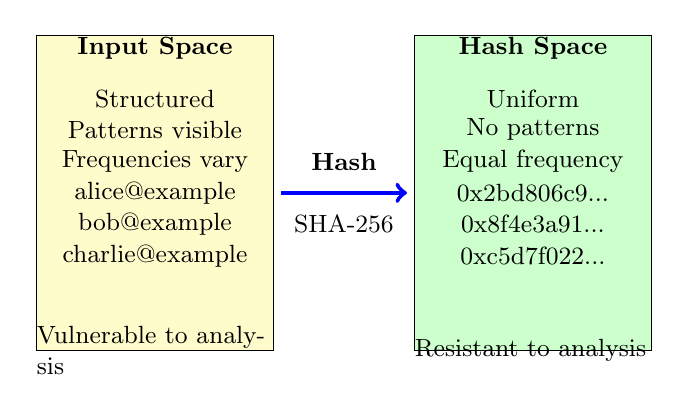
\begin{tikzpicture}[scale=0.8, every node/.style={font=\small}]
    % Input space
    \node[rectangle,draw,fill=yellow!20,minimum width=3cm,minimum height=4cm] (input) at (0,0) {};
    \node at (0,2.3) {\textbf{Input Space}};
    \node at (0,1.5) {Structured};
    \node at (0,1) {Patterns visible};
    \node at (0,0.5) {Frequencies vary};
    \node at (0,0) {alice@example};
    \node at (0,-0.5) {bob@example};
    \node at (0,-1) {charlie@example};
    
    % Hash function
    \draw[->,ultra thick,blue] (2,0) -- (4,0);
    \node at (3,0.5) {\textbf{Hash}};
    \node at (3,-0.5) {SHA-256};
    
    % Hash space
    \node[rectangle,draw,fill=green!20,minimum width=3cm,minimum height=4cm] (hash) at (6,0) {};
    \node at (6,2.3) {\textbf{Hash Space}};
    \node at (6,1.5) {Uniform};
    \node at (6,1) {No patterns};
    \node at (6,0.5) {Equal frequency};
    \node at (6,0) {0x2bd806c9...};
    \node at (6,-0.5) {0x8f4e3a91...};
    \node at (6,-1) {0xc5d7f022...};
    
    % Annotations
    \node[text width=3cm] at (0,-2.5) {Vulnerable to analysis};
    \node[text width=3cm] at (6,-2.5) {Resistant to analysis};
\end{tikzpicture}
\end{center}

\subsection{Distribution Transformation}

\begin{center}
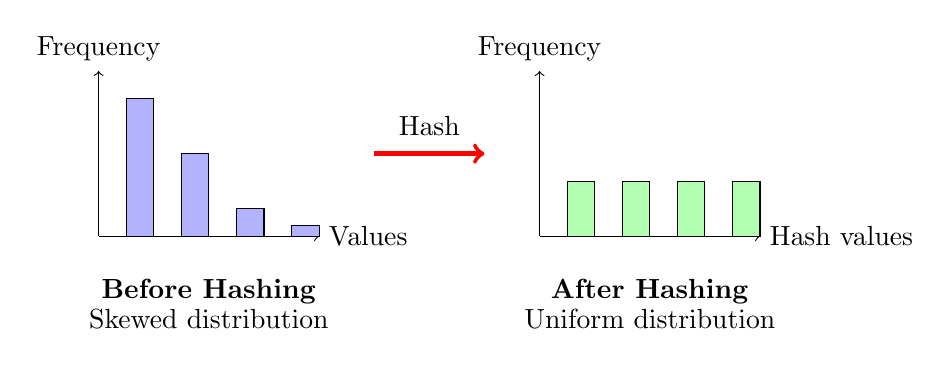
\begin{tikzpicture}[scale=0.7]
    % Before hashing - skewed distribution
    \begin{scope}[shift={(0,0)}]
        \draw[->] (0,0) -- (4,0) node[right] {Values};
        \draw[->] (0,0) -- (0,3) node[above] {Frequency};
        \node at (2,-1) {\textbf{Before Hashing}};
        
        \draw[fill=blue!30] (0.5,0) rectangle (1,2.5);
        \draw[fill=blue!30] (1.5,0) rectangle (2,1.5);
        \draw[fill=blue!30] (2.5,0) rectangle (3,0.5);
        \draw[fill=blue!30] (3.5,0) rectangle (4,0.2);
        
        \node at (2,-1.5) {Skewed distribution};
    \end{scope}
    
    % Arrow
    \draw[->,ultra thick,red] (5,1.5) -- (7,1.5);
    \node at (6,2) {Hash};
    
    % After hashing - uniform distribution
    \begin{scope}[shift={(8,0)}]
        \draw[->] (0,0) -- (4,0) node[right] {Hash values};
        \draw[->] (0,0) -- (0,3) node[above] {Frequency};
        \node at (2,-1) {\textbf{After Hashing}};
        
        \draw[fill=green!30] (0.5,0) rectangle (1,1);
        \draw[fill=green!30] (1.5,0) rectangle (2,1);
        \draw[fill=green!30] (2.5,0) rectangle (3,1);
        \draw[fill=green!30] (3.5,0) rectangle (4,1);
        
        \node at (2,-1.5) {Uniform distribution};
    \end{scope}
\end{tikzpicture}
\end{center}

\section{Hashing in Bloom Filters Revisited}

Now we can understand why Bloom filters work so well for privacy:

\begin{enumerate}
    \item \textbf{Input transformation}: Elements are hashed to uniform positions
    \item \textbf{Pattern destruction}: Related inputs map to unrelated positions
    \item \textbf{Information hiding}: The bit array reveals nothing about elements
    \item \textbf{Plausible deniability}: False positives provide cover
\end{enumerate}

\begin{example}[Privacy-Preserving Email Check]
Let's revisit our email breach checker with privacy in mind:

\begin{lstlisting}[language=C++]
class PrivateBreachChecker {
    BitArray bits(12'000'000);
    uint64_t seed;  // Secret seed
    
    uint64_t hash_with_seed(const string& email, int function_id) {
        // Combine email with seed and function ID
        string input = email + to_string(seed) + to_string(function_id);
        return sha256(input);
    }
    
    bool check(const string& email_hash) {
        // Client sends hash, not email
        // Server can't recover email from hash
        for (int i = 0; i < 3; i++) {
            if (!bits[hash_with_seed(email_hash, i) % bits.size()]) {
                return false;
            }
        }
        return true;
    }
};
\end{lstlisting}

The server never sees actual emails, only hashes that look random!
\end{example}

\section{The Bridge to Oblivious Computing}

Hashing creates uniformity, but by itself isn't enough for privacy. The key insight: combine hashing with Bernoulli approximation.

\subsection{The Two-Part Recipe}

\begin{enumerate}
    \item \textbf{Hashing}: Transform inputs to uniform distribution
    \item \textbf{Approximation}: Add controlled errors for plausible deniability
\end{enumerate}

Together, they create \emph{oblivious} data structures where:
\begin{itemize}
    \item All values look uniformly random
    \item Operations still work (with controlled error)
    \item Observers learn nothing about actual data
\end{itemize}

\subsection{Preview: The Oblivious Transform}

Here's a preview of where we're heading:

\begin{lstlisting}[language=C++]
// Standard Bloom filter (not private)
BloomFilter bf;
bf.insert("alice@example.com");
bool contains = bf.contains("alice@example.com");

// Oblivious Bloom filter (private)
ObliviousBloomFilter obf(secret_key);
auto encrypted_query = obf.encode("alice@example.com");
auto encrypted_response = obf.contains(encrypted_query);
bool result = obf.decode(encrypted_response);
\end{lstlisting}

The oblivious version:
\begin{itemize}
    \item Queries look like random hashes
    \item Responses are indistinguishable from random
    \item Yet functionality is preserved (with same error rate)
\end{itemize}

\section{Chapter Summary and Exercises}

We've discovered that:
\begin{itemize}
    \item Hash functions transform structured data into uniform randomness
    \item Uniform distributions maximize entropy and therefore privacy
    \item The maximum entropy principle guides privacy-preserving design
    \item Combining hashing with approximation enables oblivious computing
\end{itemize}

Next chapter, we'll explore what adversaries can observe and why traditional approaches fail to protect privacy.

\subsection{Exercises}

\begin{enumerate}
    \item \textbf{Entropy Calculation}: Calculate the entropy of:
    \begin{itemize}
        \item A biased coin with $P(\text{heads}) = 0.7$
        \item A die weighted so $P(6) = 0.5$ and other faces equal
        \item The English alphabet with actual letter frequencies
    \end{itemize}
    
    \item \textbf{Hash Uniformity}: Write a program to verify that SHA-256 produces approximately uniform outputs. Hash 1 million sequential integers and check the distribution of first bytes.
    
    \item \textbf{Avalanche Effect}: Implement a function to measure the avalanche effect: on average, how many output bits change when one input bit changes?
    
    \item \textbf{Frequency Hiding}: Design an encoding scheme that hides the frequency distribution of the top 10 Google searches. How many encodings does each term need?
    
    \item \textbf{Maximum Entropy}: Prove that the uniform distribution maximizes entropy for a discrete random variable over $n$ values.
    
    \item \textbf{Information Leakage}: If a hash function produces 256-bit outputs but an adversary observes that outputs always have exactly 128 ones and 128 zeros, how much information is leaked? Calculate the entropy loss.
    
    \item \textbf{Collision Birthday}: For a hash function with $n$-bit output, approximately how many random inputs must be hashed before expecting a collision? Why is this called the birthday paradox?
    
    \item \textbf{Implementation Challenge}: Build a simple privacy-preserving set membership test using hashing. The server should learn nothing about client queries.
\end{enumerate}

\subsection{Further Reading}

\begin{itemize}
    \item Shannon, C. E. (1948). "A mathematical theory of communication"
    \item Jaynes, E. T. (1957). "Information theory and statistical mechanics"
    \item Rogaway, P., \& Shrimpton, T. (2004). "Cryptographic hash-function basics"
    \item Cover, T. M., \& Thomas, J. A. (2006). "Elements of Information Theory"
\end{itemize}

\begin{researchfrontier}
Can we characterize exactly when the random oracle model is a safe assumption? What properties of real hash functions are sufficient for privacy-preserving applications?
\end{researchfrontier}